\documentclass{standalone}
\usepackage{tikz}
\usetikzlibrary{patterns, positioning}


\begin{document}
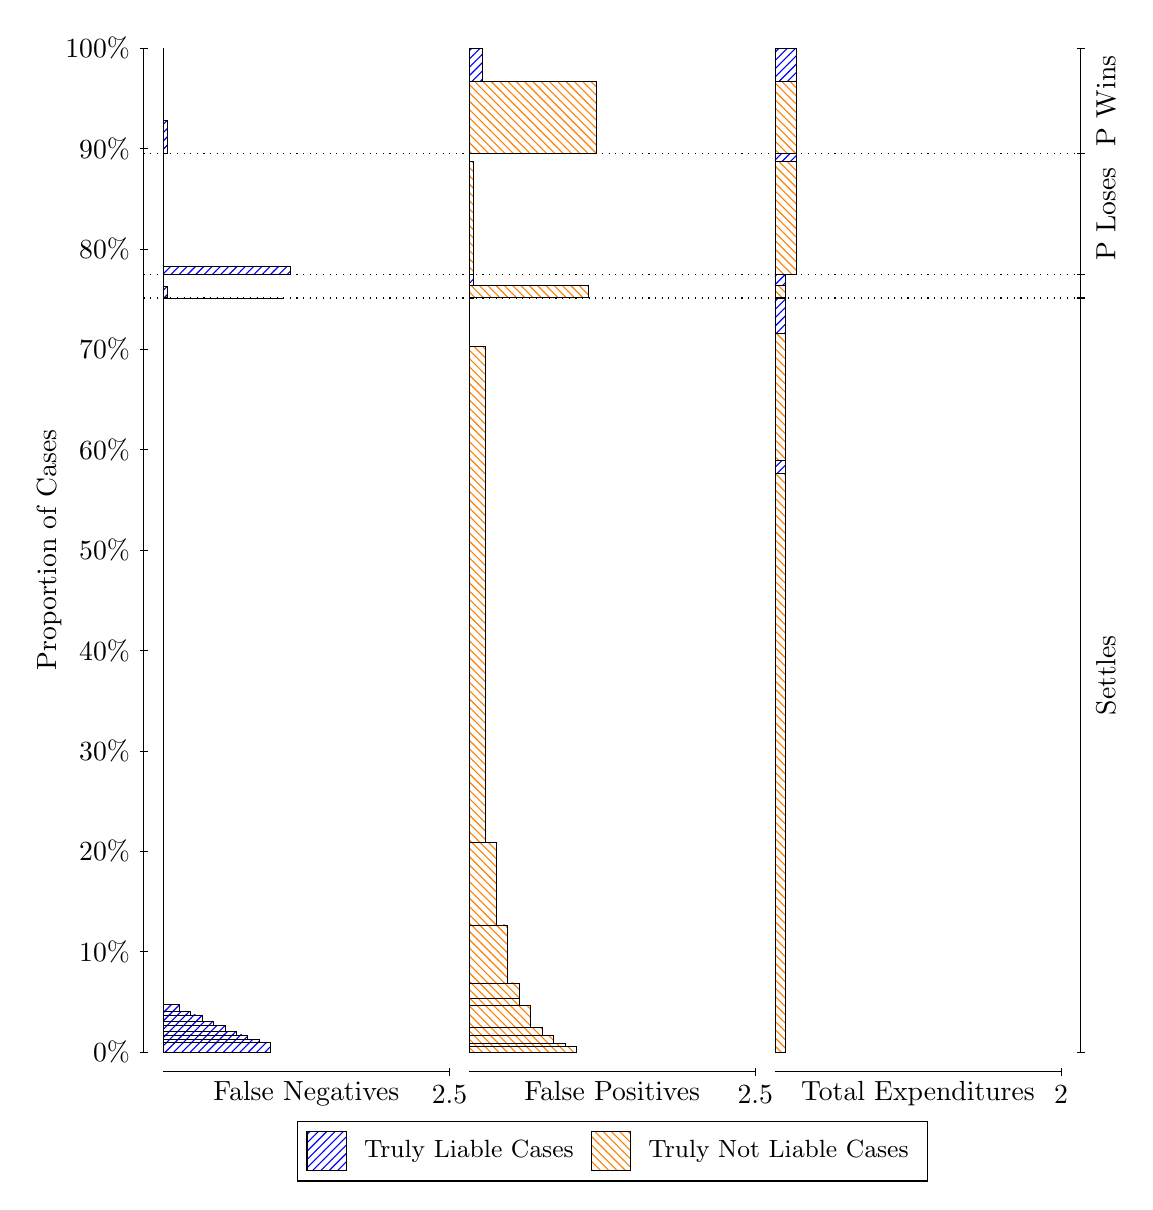
\begin{tikzpicture}
\draw[black, very thin] (1.5,1.75) -- (1.5,14.5);
\node[rotate=90, text=black, anchor=center] at (0.3, 8.125) {Proportion of Cases};
\draw[black, very thin] (1.45,1.75) -- (1.55,1.75);
\node[text=black, anchor=east] at (1.45, 1.75) {0\%};
\draw[black, very thin] (1.45,3.025) -- (1.55,3.025);
\node[text=black, anchor=east] at (1.45, 3.025) {10\%};
\draw[black, very thin] (1.45,4.3) -- (1.55,4.3);
\node[text=black, anchor=east] at (1.45, 4.3) {20\%};
\draw[black, very thin] (1.45,5.575) -- (1.55,5.575);
\node[text=black, anchor=east] at (1.45, 5.575) {30\%};
\draw[black, very thin] (1.45,6.85) -- (1.55,6.85);
\node[text=black, anchor=east] at (1.45, 6.85) {40\%};
\draw[black, very thin] (1.45,8.125) -- (1.55,8.125);
\node[text=black, anchor=east] at (1.45, 8.125) {50\%};
\draw[black, very thin] (1.45,9.4) -- (1.55,9.4);
\node[text=black, anchor=east] at (1.45, 9.4) {60\%};
\draw[black, very thin] (1.45,10.675) -- (1.55,10.675);
\node[text=black, anchor=east] at (1.45, 10.675) {70\%};
\draw[black, very thin] (1.45,11.95) -- (1.55,11.95);
\node[text=black, anchor=east] at (1.45, 11.95) {80\%};
\draw[black, very thin] (1.45,13.225) -- (1.55,13.225);
\node[text=black, anchor=east] at (1.45, 13.225) {90\%};
\draw[black, very thin] (1.45,14.5) -- (1.55,14.5);
\node[text=black, anchor=east] at (1.45, 14.5) {100\%};

\draw[black, very thin] (13.4,1.75) -- (13.4,14.5);
\draw[black, very thin] (13.35,1.75) -- (13.45,1.75);
\node[anchor=west] at (13.35, 1.75) {};
\draw[black, very thin] (13.35,11.318) -- (13.45,11.318);
\node[anchor=west] at (13.35, 11.318) {};
\draw[black, very thin] (13.35,11.334) -- (13.45,11.334);
\node[anchor=west] at (13.35, 11.334) {};
\draw[black, very thin] (13.35,11.626) -- (13.45,11.626);
\node[anchor=west] at (13.35, 11.626) {};
\draw[black, very thin] (13.35,13.158) -- (13.45,13.158);
\node[anchor=west] at (13.35, 13.158) {};
\draw[black, very thin] (13.35,14.5) -- (13.45,14.5);
\node[anchor=west] at (13.35, 14.5) {};

\draw[black, very thin, pattern color=blue, pattern=north east lines] (1.75,1.75) rectangle (3.1125,1.8693);
\draw[black, very thin, pattern color=blue, pattern=north east lines] (1.75,1.8693) rectangle (2.9672,1.9082);
\draw[black, very thin, pattern color=blue, pattern=north east lines] (1.75,1.9082) rectangle (2.8218,1.9675);
\draw[black, very thin, pattern color=blue, pattern=north east lines] (1.75,1.9675) rectangle (2.6765,2.0126);
\draw[black, very thin, pattern color=blue, pattern=north east lines] (1.75,2.0126) rectangle (2.5312,2.0926);
\draw[black, very thin, pattern color=blue, pattern=north east lines] (1.75,2.0926) rectangle (2.3858,2.1401);
\draw[black, very thin, pattern color=blue, pattern=north east lines] (1.75,2.1401) rectangle (2.2405,2.2204);
\draw[black, very thin, pattern color=blue, pattern=north east lines] (1.75,2.2204) rectangle (2.0952,2.2609);
\draw[black, very thin, pattern color=blue, pattern=north east lines] (1.75,2.2609) rectangle (1.9498,2.3529);
\draw[black, very thin, pattern color=orange, pattern=north west lines] (1.75,2.3529) rectangle (1.75,11.318);
\draw[black, very thin, pattern color=blue, pattern=north east lines] (1.75,11.318) rectangle (3.2578,11.319);
\draw[black, very thin, pattern color=orange, pattern=north west lines] (1.75,11.319) rectangle (1.75,11.334);
\draw[black, very thin, pattern color=blue, pattern=north east lines] (1.75,11.334) rectangle (1.8045,11.477);
\draw[black, very thin, pattern color=orange, pattern=north west lines] (1.75,11.477) rectangle (1.75,11.626);
\draw[black, very thin, pattern color=blue, pattern=north east lines] (1.75,11.626) rectangle (3.3668,11.726);
\draw[black, very thin, pattern color=orange, pattern=north west lines] (1.75,11.726) rectangle (1.75,13.158);
\draw[black, very thin, pattern color=blue, pattern=north east lines] (1.75,13.158) rectangle (1.8045,13.585);
\draw[black, very thin, pattern color=orange, pattern=north west lines] (1.75,13.585) rectangle (1.75,14.5);
\draw[black, very thin, pattern color=orange, pattern=north west lines] (5.6333,1.75) rectangle (6.9958,1.8189);
\draw[black, very thin, pattern color=orange, pattern=north west lines] (5.6333,1.8189) rectangle (6.8505,1.8544);
\draw[black, very thin, pattern color=orange, pattern=north west lines] (5.6333,1.8544) rectangle (6.7052,1.9618);
\draw[black, very thin, pattern color=orange, pattern=north west lines] (5.6333,1.9618) rectangle (6.5598,2.0672);
\draw[black, very thin, pattern color=orange, pattern=north west lines] (5.6333,2.0672) rectangle (6.4145,2.3384);
\draw[black, very thin, pattern color=orange, pattern=north west lines] (5.6333,2.3384) rectangle (6.2692,2.4271);
\draw[black, very thin, pattern color=orange, pattern=north west lines] (5.6333,2.4271) rectangle (6.2692,2.6274);
\draw[black, very thin, pattern color=orange, pattern=north west lines] (5.6333,2.6274) rectangle (6.1238,3.3637);
\draw[black, very thin, pattern color=orange, pattern=north west lines] (5.6333,3.3637) rectangle (5.9785,4.4127);
\draw[black, very thin, pattern color=orange, pattern=north west lines] (5.6333,4.4127) rectangle (5.8332,10.715);
\draw[black, very thin, pattern color=blue, pattern=north east lines] (5.6333,10.715) rectangle (5.6333,11.318);
\draw[black, very thin, pattern color=orange, pattern=north west lines] (5.6333,11.318) rectangle (5.6878,11.333);
\draw[black, very thin, pattern color=blue, pattern=north east lines] (5.6333,11.333) rectangle (5.6333,11.334);
\draw[black, very thin, pattern color=orange, pattern=north west lines] (5.6333,11.334) rectangle (7.1412,11.483);
\draw[black, very thin, pattern color=blue, pattern=north east lines] (5.6333,11.483) rectangle (5.6878,11.626);
\draw[black, very thin, pattern color=orange, pattern=north west lines] (5.6333,11.626) rectangle (5.6878,13.058);
\draw[black, very thin, pattern color=blue, pattern=north east lines] (5.6333,13.058) rectangle (5.6333,13.158);
\draw[black, very thin, pattern color=orange, pattern=north west lines] (5.6333,13.158) rectangle (7.2502,14.073);
\draw[black, very thin, pattern color=blue, pattern=north east lines] (5.6333,14.073) rectangle (5.7968,14.5);
\draw[black, very thin, pattern color=orange, pattern=north west lines] (9.5167,1.75) rectangle (9.6529,9.1013);
\draw[black, very thin, pattern color=blue, pattern=north east lines] (9.5167,9.1013) rectangle (9.6529,9.2595);
\draw[black, very thin, pattern color=orange, pattern=north west lines] (9.5167,9.2595) rectangle (9.6529,10.873);
\draw[black, very thin, pattern color=blue, pattern=north east lines] (9.5167,10.873) rectangle (9.6529,11.318);
\draw[black, very thin, pattern color=orange, pattern=north west lines] (9.5167,11.318) rectangle (9.6529,11.333);
\draw[black, very thin, pattern color=blue, pattern=north east lines] (9.5167,11.333) rectangle (9.6529,11.334);
\draw[black, very thin, pattern color=orange, pattern=north west lines] (9.5167,11.334) rectangle (9.6529,11.483);
\draw[black, very thin, pattern color=blue, pattern=north east lines] (9.5167,11.483) rectangle (9.6529,11.626);
\draw[black, very thin, pattern color=orange, pattern=north west lines] (9.5167,11.626) rectangle (9.7892,13.058);
\draw[black, very thin, pattern color=blue, pattern=north east lines] (9.5167,13.058) rectangle (9.7892,13.158);
\draw[black, very thin, pattern color=orange, pattern=north west lines] (9.5167,13.158) rectangle (9.7892,14.073);
\draw[black, very thin, pattern color=blue, pattern=north east lines] (9.5167,14.073) rectangle (9.7892,14.5);
\draw[black, dotted] (1.5,11.318) -- (13.4,11.318);
\draw[black, dotted] (1.5,11.334) -- (13.4,11.334);
\draw[black, dotted] (1.5,11.626) -- (13.4,11.626);
\draw[black, dotted] (1.5,13.158) -- (13.4,13.158);
\draw[black, very thin] (1.75,1.5) -- (5.3833,1.5);
\node[text=black, anchor=north] at (3.5667, 1.5) {False Negatives};
\draw[black, very thin] (5.3833,1.45) -- (5.3833,1.55);
\node[text=black, anchor=north] at (5.3833, 1.45) {2.5};

\draw[black, very thin] (5.6333,1.5) -- (9.2667,1.5);
\node[text=black, anchor=north] at (7.45, 1.5) {False Positives};
\draw[black, very thin] (9.2667,1.45) -- (9.2667,1.55);
\node[text=black, anchor=north] at (9.2667, 1.45) {2.5};

\draw[black, very thin] (9.5167,1.5) -- (13.15,1.5);
\node[text=black, anchor=north] at (11.333, 1.5) {Total Expenditures};
\draw[black, very thin] (13.15,1.45) -- (13.15,1.55);
\node[text=black, anchor=north] at (13.15, 1.45) {2};

\node[text=black, centered, rotate=90] at (13.72, 6.5339) {Settles};


\node[text=black, centered, rotate=90] at (13.72, 12.392) {P Loses};
\node[text=black, centered, rotate=90] at (13.72, 13.829) {P Wins};

\draw (7.449999999999999,1.5) node[draw=none] (baseCoordinate) {};
\begin{scope}[align=center]
        \matrix[scale=0.5, draw=black, below=0.5cm of baseCoordinate, nodes={draw}, column sep=0.1cm]{
            \node[rectangle, draw, minimum width=0.5cm, minimum height=0.5cm, pattern color=blue, pattern=north east lines] {}; &
            \node[draw=none, font=\small, text=black] (B) {Truly Liable Cases}; &
            \node[rectangle, draw, minimum width=0.5cm, minimum height=0.5cm, pattern color=orange, pattern=north west lines] {}; &
            \node[draw=none, font=\small, text=black] (B) {Truly Not Liable Cases}; \\
            };
\end{scope}

\end{tikzpicture}
\end{document}